\section{Power Supplies}

\begin{center}
\textit{Power Supplies 1}
\vspace{1mm}
\hrule
\end{center}

\subsection{What \textit{is} power?}

Power is the rate of disapation of energy. You can express power in terms of voltage and current using the chain rule.

\begin{align*}
P = \frac{dE}{dt},\, V = \frac{dP}{dQ},\, I = \frac{dQ}{dt}
\end{align*}

\begin{align*}
P = I \cdot V = \frac{dP}{dQ} \cdot \frac{dQ}{dt} = \frac{dE}{dt}
\end{align*}

Losses are often expressed in terms of power. Ohmic loss is the power lost though resistance. 

\begin{align*}
P = I^2R
\end{align*}

This means that to decrease Ohmic loss you can increase the voltage while decreasing the current. This is easy to do for AC with a transformer, but harder to achieve for DC.

\subsection{Quantifying Time-dependent Voltage}

\begin{itemize}
	\item Instantaneous value
	\item Peak value
	\item Peak to peak value
	\item Average value
	\item Effective value or RMS
\end{itemize}

\subsubsection{Effective Voltage and Power}

\begin{gather*}
\textrm{At DC:}\; P = IV = \frac{V^2}{R} \\
\textrm{At AC:}\; P_{AV} = \frac{1}{T} \int^T_0 \frac{v^2(t)}{R} dt
\end{gather*}

$V_{RMS}$ is a voltage that will cause the same loss in a resistance $R$ as a DC voltage $V$.

\begin{gather*}
P_{AV} = \frac{V^2_{RMS}}{R} = \frac{1}{T}\int^T_0 \frac{v^2(t)}{R}dt \\
\downarrow \\
V_{RMS} = \sqrt{\frac{1}{T}\int^T_0v^2(t)dt} \\
\end{gather*}

For a generic AC voltage $V_m\sin(\omega t)$ this solves to the following.

\begin{align*}
V_{RMS} &= \frac{1}{2\pi} \int^{2\pi}_{0} V_m^2 \sin^2(\omega t) d(\omega t) \\
        &= \frac{V_m^2}{4\pi} \int^{2\pi}_{0}  (1 - \cos(\omega t)) d(\omega t) \\
V_{RMS} &= \frac{V_m}{2}
\end{align*}

\subsection{Transformers}

Transformers convert AC voltages. This conversion is done in the ratio of turns in each coil: the turn ratio $a$.

\begin{equation*}
a = \frac{n_1}{n_2} = \frac{v_1}{v_2}
\end{equation*}

\subsection{Rectification}

Rectification is the process of converting AC $\rightarrow$ DC voltages.

\subsubsection{Half Wave Rectifier}

In a half wave rectifier a diode is used to remove the negative part of the signal over a load 

\begin{figure}[H]
\centering
\href{https://en.wikipedia.org/wiki/Rectifier#/media/File:Halfwave.rectifier.en.svg}{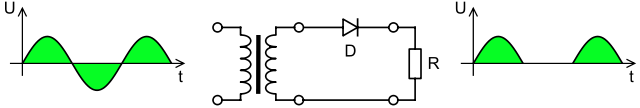
\includegraphics[width=\textwidth]{images/half-wave-rectifier.png}}
\caption{Circuit, input and output diagrams for a half-wave rectifier.}
\end{figure}

You can then put a capacitor across the output to smoothen the output waveform.

\subsubsection{Full Wave Rectifier}

Using a center tap on the transformer you can do full wave rectification.

\begin{figure}[H]
\centering
\href{https://en.wikipedia.org/wiki/Rectifier#/media/File:Fullwave.rectifier.en.svg}{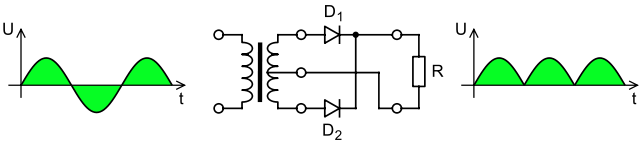
\includegraphics[width=\textwidth]{images/full-wave-rectifier.png}}
\caption{Circuit, input and output diagrams for a full-wave rectifier.}
\end{figure}

\subsubsection{Bridge Rectifier}

A bridge rectifier doesn't require a center tap on the transformer, and has half the current though the diodes, but has twice the voltage drop though the resistors.

\begin{figure}[H]
\centering
\href{https://en.wikipedia.org/wiki/Rectifier#/media/File:Gratz.rectifier.en.svg}{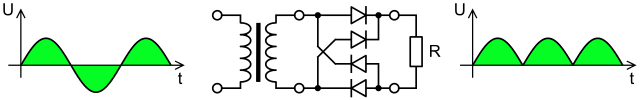
\includegraphics[width=\textwidth]{images/bridge-rectifier.png}}
\caption{Circuit, input and output diagrams for a bridge rectifier.}
\end{figure}

\subsection{Quantifying and Calculating Ripple Voltage}

Ripple voltage is the deviation from the ideal DC voltage at the output. The voltage decay from the maximum voltage can be expressed as the following:

\begin{gather*}
v_0(t) = v_p e^{-\frac{t}{RC}}
\end{gather*}

Then using the fact that for small $t$, $e^{-x} \approx 1-x$:

\begin{gather*}
v_{min} = v_p\left(1 - \frac{t}{RC}\right)
\end{gather*}

Then if $RC >> T$:

\begin{gather*}
v_r \approx \frac{v_p T}{RC}
\end{gather*}

\begin{framed}
\textbf{What capacitance is required for a less then 5\% ripple in a Half Wave Rectifier over a load of 16k$\Omega$?}
\begin{align*}
v_r &= \frac{v_pT}{RC} \\
\frac{v_r}{v_p} &= \frac{T}{RC} \\
\frac{T}{RC} &= 5\% \\
C &= \frac{T}{0.05 \cdot R} = 25\mu\textrm{F}
\end{align*}
\end{framed}

From the above example you can see that a larger capacitance gives a smaller ripple. But large capacitors get expensive. It might be worth trying a regulator...

\subsection{Regulators}

\begin{itemize}
	\item Line Regulation - keeping a constant output voltage with a varying input voltage.
	\item Load Regulation - keeping a constant output voltage with a varying output load.
	\item Ripple Rejection
\end{itemize}

\subsubsection{Quantifying Power Supply Efficiency}

\begin{itemize}
	\item Quiescent Current is the current used by the supply at idle.
	\item Efficiency, $P_{out} / P_{in}$, is normally a large percentage.
\end{itemize}

\subsubsection{Linear vs Switching Regulators}

\begin{table}[H]
	\centering
	\caption{Tabulated differences between Linear and Switching regulators.}
    \begin{tabular}{ll}
    Linear & Switching \\
    \hline
    Operates in linear region & Operates as a switch \\
    Simple & Complex \\
    Inefficient & Efficient
    \end{tabular}
\end{table}

Additionally to the table above:

\begin{itemize}
	\item Linear regulators are stable, resulting in a small $v_r$, but are step-down only.
	\item Switching regulators are more flexible then linear ones are they can be both boost (step-up) and buck (step-down) or boost-buck, however, they produce a lot of noise due to their switching nature.
\end{itemize}

\subsection{Types of Linear Regulator}

\subsubsection{Series Regulator}

A series regulator is (shock) placed in series with the voltage source. It has three pins, $v_{in}$, $v_{out}$ and \texttt{GND}.

\begin{figure}[H]
\centering
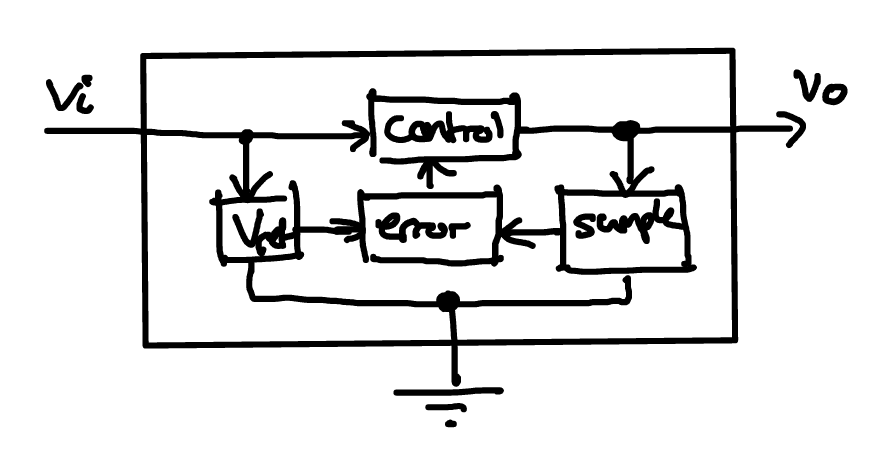
\includegraphics[width=0.5\textwidth]{images/linear-reg.png}
\caption{Block diagram for a series linear regulator.}
\end{figure}

Inside the regulator are four main components. 

\begin{itemize}
    \item $v_{ref}$, a voltage reference, normally a Zener diode.
    \item An error block, which is physically an op-amp.
    \item A sample stage, which is just a voltage divider.
    \item A Control element, physically a transistor.
\end{itemize}

\subsubsection{Shunt Regulator}

A shunt regulator is similar to a series regulator but is placed in parallel with the load. 

\begin{figure}[H]
\centering
\href{http://www.ti.com/product/LM431/datasheet}{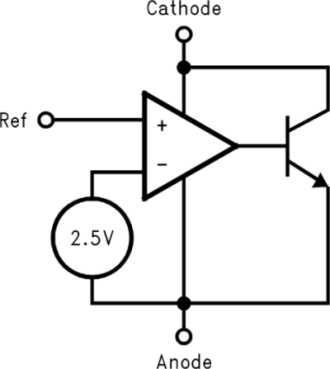
\includegraphics[width=0.25\textwidth]{images/shunt-reg.png}}
\caption{Schematic of TI's LM431 shunt voltage regulator.}
\end{figure}

\subsection{Heat Flow in Linear Regulators}

\begin{framed}
\textbf{In a linear regulator dropping from 8V to 3V with a current of 1A, how much power must be dissipated in the regulator?}
\begin{align*}
P &= IV \\
P &= 1\cdot(8-5) \\
P &= 3\textrm{W}
\end{align*}
\end{framed}

As shown in the above example a lot of power, and therefore heat, is generated in a linear regulator. To remove this heat from the board we use a heat sink.

The maximum temperature a silicon semiconductor will work at is roughly 150 to 200 \degree C.

\subsection{Modeling Heat Flow}

\begin{align*}
\Delta T = P_j \theta
\end{align*}

Where:

\begin{table}[H]
	\centering
    \begin{tabular}{lll}
    $\Delta T$ & is the temperature difference. \\
    $P_j$      & is the power dissipated at the junction. \\
    $\theta$   & is the thermal resistance, in kelvin per watt, $\frac{K}{W}$. \\
    \end{tabular}
\end{table}

Normally the heat will flow though several boundaries. This requires you to equate several thermal resistances, for example the junction to case, $\theta_{jc}$ and case to ambient, $\theta_{ca}$.

\begin{gather*}
T_j - T_c = \theta_{jc}P_j \\
T_c - T_a = \theta_{ca}P_j \\
\downarrow \\
T_j = T_a + (\theta_{jc} + \theta_{ca})P_j
\end{gather*}

This can be concidered a general form, so adding a heat sink on the case would lead to the following:

\begin{gather*}
T_j = T_a + (\theta_{jc} + \theta_{cs} + \theta_{sa})P_j
\end{gather*}

\begin{framed}
\textbf{For a 3W transistor with the following thermal resistances, what is the junction temperature in a 25\degree C room?}
\begin{table}[H]
	\centering
    \begin{tabular}{lll}
    $\theta_{jc}$ & of 5 K/W \\
    $\theta_{cs}$ & of 2 K/W \\
    $\theta_{sa}$ & of 10 K/W
    \end{tabular}
\end{table}
\begin{align*}
T_j &= T_a + (\theta_{jc} + \theta_{cs} + \theta_{sa})P_j \\
    &= 25 + (5 + 2 + 10) \times 3 \\
    &= 25 + 17 \times 3 \\
T_j &= 76\degree C
\end{align*}
\end{framed}